

\setcounter{section}{1}
\section{Break-Even Analysis}

\bigskip
Break-even analysis details the calculation for the margin of safety for the Akriveia Beacon based on the revenues collected and associated costs [4]. By analyzing different price levels relating to various levels of demand, the break-even analysis can determine the level of sales necessary to cover the company's total fixed costs. Break-even analysis depends on the Break-even Point (BEP) which is calculated by dividing the total fixed costs of production by the contribution margin or price difference of a product per individual unit and the variable costs of production as shown in equation (1) [5]. 

\begin{equation}
	\text{BEP = Fixed Costs / ( Selling Price - Variable Cost Per Unit )}
\end{equation}

There are two phases where the break-even point will be calculated for, first is the gamma prototype which reflects the current product state, the second will be the mass production version which reflects the final version of the Akriveia Beacon at a higher level of optimization with integrated PCB and injection molding casing design. For mass production a quantity of 1000 is used for quoting.

\subsection{Gamma Prototype}

\medskip
For Gamma Prototype the fix cost is fairly low as there are no cost associated with tangible or intangible assets, rent, salaries, utilities, and taxes; since the development team is composed of SFU engineering students. To simply calculations the fix cost will be determined by the amount of budget current contributed to the development of the prototype which will be \$1000.00 CAD. Component cost for each beacon and ID Tag is shown below in Table 1 and Table 2. These costs reflect the purchase price of each component on the date of purchase and are derived only from material costs, which does not include additional costs such as shipping, import taxes, labour, and miscellaneous materials used such as wires, solder, screws, tape, and etc, since materials were obtained outside of budget. Furthermore, software development cost is considered to be zero.

\bgroup
\def\arraystretch{1.5}
\begin{table}[H]
\centering
\begin{tabular}{ | m{9.75cm} | m{3.25cm} | m{2.5cm} |}
\hline
\textbf{Item} & \textbf{Supplier} & \textbf{Price [CAD]}\\
\hline
DWM1000 UWB RF TX/RX MODULE {[6]} & Decawave & \multicolumn{1}{r|}{\$46.13} \\
\hline
Arduino Pro Mini 328 - 3.3V/8MHz {[7]} & Lonten & \multicolumn{1}{r|}{\$1.80} \\
\hline
ESP32 Development Board - ESP32-D0WDQ6 Chip [8] & WalFront & \multicolumn{1}{r|}{\$15.59} \\
\hline
DC5.0V 10000mAh Rechargeable Li-Polymer Battery & uxcell & \multicolumn{1}{r|}{\$15.99} \\
\hline
AMS1117-3.3 DC Voltage Regulator Step Down Module & Icstation & \multicolumn{1}{r|}{\$2.40} \\
\hline
Power Hexfet IRFZ44 N-Channel $\times$2 & Infineon & \multicolumn{1}{r|}{\$5.60} \\
\hline
Push Button PS-29C On-Off & Daywel & \multicolumn{1}{r|}{\$1.30} \\
\hline
$8\times12$cm Double Sided Universal PerfBoard [9] & uxcell & \multicolumn{1}{r|}{\$3.47} \\
\hline
Beacon Casing 3D Printing [10] & 3DHubs & \multicolumn{1}{r|}{\$35.27} \\
\hline
\multicolumn{2}{|r|}{\textbf{Total:}} & \multicolumn{1}{r|}{\textbf{\$127.55}} \\
\hline
\end{tabular}
\caption{Gamma Prototype Beacon Component \& Price}
\end{table}

\bgroup
\def\arraystretch{1.5}
\begin{table}[H]
\centering
\begin{tabular}{ | m{9.75cm} | m{3.25cm} | m{2.5cm} |}
\hline
\textbf{Item} & \textbf{Supplier} & \textbf{Price [CAD]}\\
\hline
DWM1000 UWB RF TX/RX MODULE {[6]} & Decawave & \multicolumn{1}{r|}{\$46.13} \\
\hline
Arduino Pro Mini 328 - 3.3V/8MHz {[7]} & Lonten & \multicolumn{1}{r|}{\$1.80} \\
\hline
DC3.0V 1000mAh Rechargeable Li-Polymer Battery & uxcell & \multicolumn{1}{r|}{\$10.24} \\
\hline
Micro USB 5V 1A TP4056 Battery Charger Module & NJTP ASIC Corp. & \multicolumn{1}{r|}{\$1.79} \\
\hline
Push Button PS-29C On-Off & Daywel & \multicolumn{1}{r|}{\$1.30} \\
\hline
$4\times6$cm Double Sided Universal PerfBoard [9] & uxcell & \multicolumn{1}{r|}{\$1.41} \\
\hline
Beacon Casing 3D Printing [10] & 3DHubs & \multicolumn{1}{r|}{\$11.89} \\
\hline
\multicolumn{2}{|r|}{\textbf{Total:}} & \multicolumn{1}{r|}{\textbf{\$74.56}} \\
\hline
\end{tabular}
\caption{Gamma Prototype ID Tag Component \& Price}
\end{table}

Since the Akriveia Beacon product is meant to be sold as a system and not an individual product, multiple Beacons and ID Tags must be purchased as a package. Assuming each package/unit of purchase contains 3 Beacons and 10 ID tags along with an estimated software lease cost of \$250, and a desired return on sales of 25\% (excluding taxes); the required sale price is calculated to be \$1722.81 for each unit as shown in equation (3). Using the values obtained below the BEP is calculated in equation (3) and plotted in Figure 1. In order for the Akriveia Beacon to break-even at its Gamma prototype state, a minimal sale of \textbf{2 units} is required.

\begin{align} 
	&\text{Variable Cost Per Unit} = \$127.55 \times 3 + \$74.56 \times 10 = \$1128.25	\\
	&\text{Required Sale Price} = \$1128.25 + \$250.00 = \$1378.25 \times 1.25 = \$1722.81 \\
	&\text{BEP} = \$1000.00 / (\$1722.81 - \$1128.25) = 1.682 \approx \textbf{2}	
\end{align}

\begin{figure}[H]
\centering
    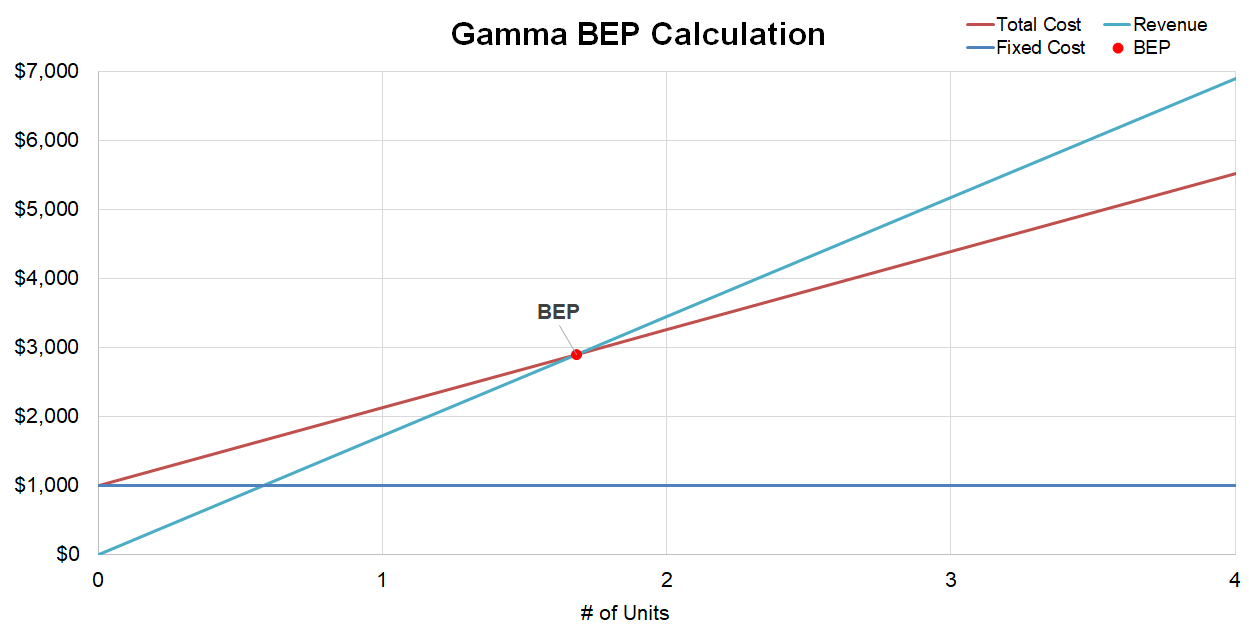
\includegraphics[width=\linewidth]{./images/gamma.png}
    \caption{Gamma Prototype Break-Even Point Calculation}
\end{figure}


\pagebreak
\subsection{Mass Production}

\medskip
For mass production the Akriveia Beacons system will undergo major design optimization including custom integrated printed circuit board (PCB) containing all hardware components, injection molding for Beacon and Tag casing and improved software deployment processes. The fixed cost is greatly increased due to various factors such as shipping, taxes, rent, utilities, labour, and office expenses. Assuming some expenses can be negated and only tooling, PCB fabrication, assembly and material costs is considered for fixed costs. 

\bigskip
Custom integrated PCB for Beacons and ID Tags will be fabricated and assembled with Arduino and ESPRESSIF integrated circuit (IC) chips ordered directly from suppliers as well as any surface mount device (SMD), which lowers the variable cost per unit dramatically. Bittele Electronics Inc. [11] was chosen as the fraborator and assembler for the integrated PCBs since they offer free passive components as part of the assembly and low prices for mass production. However, PCB assembly cost of \$3888.30 for Beacons and \$2693.32 for ID Tags will be added into fixed cost (see Appendix C). 

\bigskip
Although 3D printing is very useful for prototyping, it is not a sufficient or cost effective way for mass production. A few venders has been evaluated based on tooling price, unit cost and materials available, and 3D Hubs [10] has been chosen as the supplier for the Beacon and Tag casing which will be done through injection molding with Polyether Ether Ketone (PEEK). For injection molding there is a fix tooling cost of \$10474.79 for beacons and \$5181.55 for ID Tags (see Appendix B). Additionally, an estimate of \$2000.00 for final assembly is added, this brings the total fixed cost to \$24237.96.

\bigskip
Variable cost per unit is dramatically lowered due to bulk prices which are supplied directly from manufacturers, resulting in 71.23\% decrease in cost for Beacons and 69.45\% decrease for Tags. The mass production variable cost for Beacons and ID Tags can be seen in Table 3 and Table 4. 

\medskip
\def\arraystretch{1.5}
\begin{table}[H]
\centering
\begin{tabular}{ | m{12.5cm} | m{3cm} |}
\hline
\textbf{Item} & \textbf{Price [CAD]}\\
\hline
DWM1000 UWB RF TX/RX MODULE {[6]} & \multicolumn{1}{r|}{\$16.88} \\
\hline
PM33** & \multicolumn{1}{r|}{\$0.67} \\
\hline
ESP32** & \multicolumn{1}{r|}{\$5.72} \\
\hline
MOSFET N-Ch. 50V 500mA & \multicolumn{1}{r|}{\$0.06} \\
\hline
Linear Voltage Regulator IC 300mA & \multicolumn{1}{r|}{\$0.19} \\
\hline
TP4056 Li-ion Battery Charger IC & \multicolumn{1}{r|}{\$0.61} \\
\hline
5V 10000mAh Rechargeable Battery  & \multicolumn{1}{r|}{\$8.29} \\
\hline
30A 250VAC 1E4 Rocker Switch  & \multicolumn{1}{r|}{\$0.50} \\
\hline
PEEK Injection Molding & \multicolumn{1}{r|}{\$2.30} \\
\hline
PCB Fabrication & \multicolumn{1}{r|}{\$1.43} \\
\hline
\multicolumn{1}{|r|}{\textbf{Total:}} & \multicolumn{1}{r|}{\textbf{\$36.70}} \\
\hline
\end{tabular}
\caption{Mass Production Beacon Component \& Price}
\end{table}

\begin{flushright}
	**Detailed BOM in Appendix A.
\end{flushright}

\pagebreak
\bgroup
\def\arraystretch{1.5}
\begin{table}[H]
\centering
\begin{tabular}{ | m{12.5cm} | m{3cm} |}
\hline
\textbf{Item} & \textbf{Price [CAD]}\\
\hline
DWM1000 UWB RF TX/RX MODULE {[6]} & \multicolumn{1}{r|}{\$16.88} \\
\hline
PM33** & \multicolumn{1}{r|}{\$0.67} \\
\hline
TP4056 Li-ion Battery Charger IC & \multicolumn{1}{r|}{\$0.61} \\
\hline
3.3V 10000mAh Rechargeable Battery  & \multicolumn{1}{r|}{\$2.10} \\
\hline
30A 250VAC 1E4 Rocker Switch  & \multicolumn{1}{r|}{\$0.50} \\
\hline
PEEK Injection Molding & \multicolumn{1}{r|}{\$1.25} \\
\hline
PCB Fabrication & \multicolumn{1}{r|}{\$0.77} \\
\hline
\multicolumn{1}{|r|}{\textbf{Total:}} & \multicolumn{1}{r|}{\textbf{\$22.78}} \\
\hline

\end{tabular}
\caption{Mass Production ID Tag Component \& Price}
\end{table}

\begin{flushright}
	**Detailed BOM in Appendix A.
\end{flushright}

\bigskip
Similar to Gamma Prototype, assuming each package/unit of purchase contains 3 Beacons and 10 ID tags along with an estimated software lease cost of \$250.00, with a desired return on sales of 25\% (excluding taxes); the required sale price for the mass production product is calculated to be \$734.88 for each unit as shown in equation (6). Using the values obtained below the mass production BEP is calculated in equation (7) and plotted in Figure 2. In order for the mass production Akriveia Beacon to break-even, a minimal sale of \textbf{62 units} is required.

\begin{align} 
	&\text{Variable Cost Per Unit} = \$36.70 * 3 + \$22.78 * 10 = \$337.90	\\
	&\text{Required Sale Price} = \$336.56 + \$250.00 = \$587.90 * 1.25 = \$734.88 \\
	&\text{BEP} = \$24237.96 / (\$734.88 - \$337.90) = 61.06 \approx \textbf{62}	
\end{align}

\begin{figure}[H]
\centering
    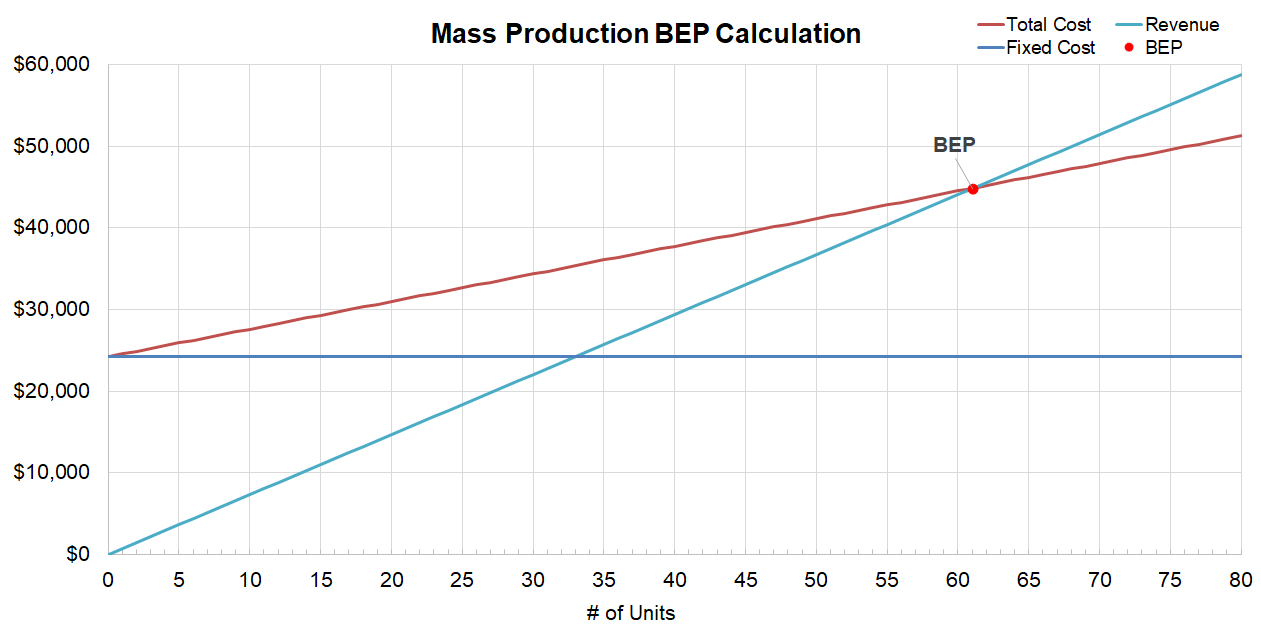
\includegraphics[width=\linewidth]{./images/mp.png}
    \caption{Mass Production Break-Even Point Calculation}
\end{figure}

